%%%%%%%%%%%%%%%%%%%%%%%%%%%%%%%%%%%%%%%%%
% Beamer Presentation
% LaTeX Template
% Version 1.0 (10/11/12)
%
% This template has been downloaded from:
% http://www.LaTeXTemplates.com
%
% License:
% CC BY-NC-SA 3.0 (http://creativecommons.org/licenses/by-nc-sa/3.0/)
%
%%%%%%%%%%%%%%%%%%%%%%%%%%%%%%%%%%%%%%%%%

%----------------------------------------------------------------------------------------
%	PACKAGES AND THEMES
%----------------------------------------------------------------------------------------

\documentclass{beamer}

\mode<presentation> {

% The Beamer class comes with a number of default slide themes
% which change the colors and layouts of slides. Below this is a list
% of all the themes, uncomment each in turn to see what they look like.

%\usetheme{default}
%\usetheme{AnnArbor}
%\usetheme{Antibes}
%\usetheme{Bergen}
%\usetheme{Berkeley}
%\usetheme{Berlin}
%\usetheme{Boadilla}
%\usetheme{CambridgeUS}
%\usetheme{Copenhagen}
%\usetheme{Darmstadt}
%\usetheme{Dresden}
%\usetheme{Frankfurt}
%\usetheme{Goettingen}
%\usetheme{Hannover}
%\usetheme{Ilmenau}
%\usetheme{JuanLesPins}
%\usetheme{Luebeck}
\usetheme{Madrid}
%\usetheme{Malmoe}
%\usetheme{Marburg}
%\usetheme{Montpellier}
%\usetheme{PaloAlto}
%\usetheme{Pittsburgh}
%\usetheme{Rochester}
%\usetheme{Singapore}
%\usetheme{Szeged}
%\usetheme{Warsaw}

% As well as themes, the Beamer class has a number of color themes
% for any slide theme. Uncomment each of these in turn to see how it
% changes the colors of your current slide theme.

%\usecolortheme{albatross}
%\usecolortheme{beaver}
%\usecolortheme{beetle}
%\usecolortheme{crane}
%\usecolortheme{dolphin}
%\usecolortheme{dove}
%\usecolortheme{fly}
%\usecolortheme{lily}
%\usecolortheme{orchid}
%\usecolortheme{rose}
%\usecolortheme{seagull}
%\usecolortheme{seahorse}
%\usecolortheme{whale}
%\usecolortheme{wolverine}

%\setbeamertemplate{footline} % To remove the footer line in all slides uncomment this line
%\setbeamertemplate{footline}[page number] % To replace the footer line in all slides with a simple slide count uncomment this line

%\setbeamertemplate{navigation symbols}{} % To remove the navigation symbols from the bottom of all slides uncomment this line
}

\usepackage{graphicx} % Allows including images
\usepackage{booktabs} % Allows the use of \toprule, \midrule and \bottomrule in tables
\usepackage{multirow}
\usepackage{xcolor}
\usepackage{amsmath}
\newcommand{\xmark}{\textcolor{red}{\text{\sffamily X}}}
\newcommand{\cmark}{\textcolor{green}{\checkmark}}
\newcommand{\tr}{\text{tr}}
\newcommand{\E}{\textbf{E}}
\newcommand{\diag}{\text{diag}}
\newcommand{\argmax}{\text{argmax}}
\newcommand{\argmin}{\text{argmin}}
\newcommand{\Cov}{\text{Cov}}
\newcommand{\Vol}{\text{Vol}}
\newcommand{\blue[1]}{\color{blue}{\textbf{#1}}}


%----------------------------------------------------------------------------------------
%	TITLE PAGE
%----------------------------------------------------------------------------------------


\title{All-Pairs-Shortest-Paths in Spark}

\author{Charles Zheng, Jingshu Wang and Arzav Jain} % Your name
\institute[Stanford] % Your institution as it will appear on the bottom of every slide, may be shorthand to save space
{Stanford University}
\date{\today} % Date, can be changed to a custom date

\begin{document}

\begin{frame}
\titlepage % Print the title page as the first slide
\end{frame}

\section{Introduction}

\begin{frame}
\frametitle{Problem}
\begin{itemize}
\item Weighted graph $G = (V, E)$ with $n$ vertices
\item Compute $n \times n$ matrix of distances $S$ where
\[
S_{ij} = \text{weight of shortest path from $i$ to $j$}
\]
\begin{center}
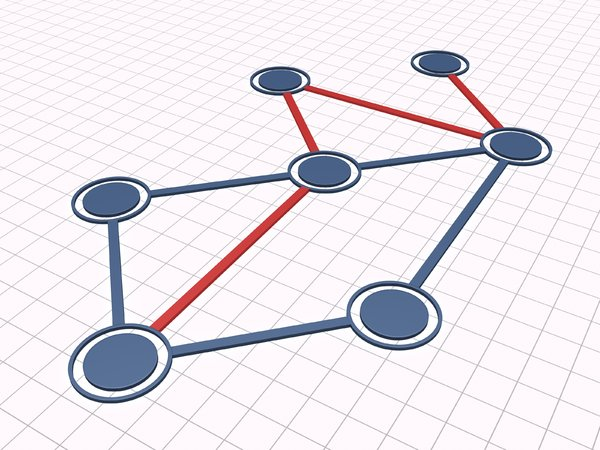
\includegraphics[scale = 0.3]{stock_sp.jpg}
\end{center}
\end{itemize}
\end{frame}

\begin{frame}
\frametitle{Floyd-Warshall: Single Core}
\vspace{3mm}
$S_{ij}^k$ - shortest path distance from $i$ to $j$ using intermediate nodes $1$ to $k$

\[
S_{ij}^k =
\begin{cases} 
      \hfill w_{ij} \hfill & k=0 \\
      \hfill min(S_{ij}^{k-1}, S_{ik}^{k-1} + S_{kj}^{k-1}) \hfill & k>0
\end{cases}
\]
\vspace{3mm}
\[
S \leftarrow min(S, S(:, k) \otimes S(k, :))
\]
\end{frame}

\begin{frame}
\frametitle{Floyd-Warshall}
Initial input
\begin{tabular}{cc}
$
\begin{pmatrix}
0&1& & & &1\\
1&0&1& & & \\
 &1&0&1& & \\
 & &1&0&1& \\
 & & &1&0&1\\
1& & & &1&0\\
\end{pmatrix}
$
&
\raisebox{-.5\height}{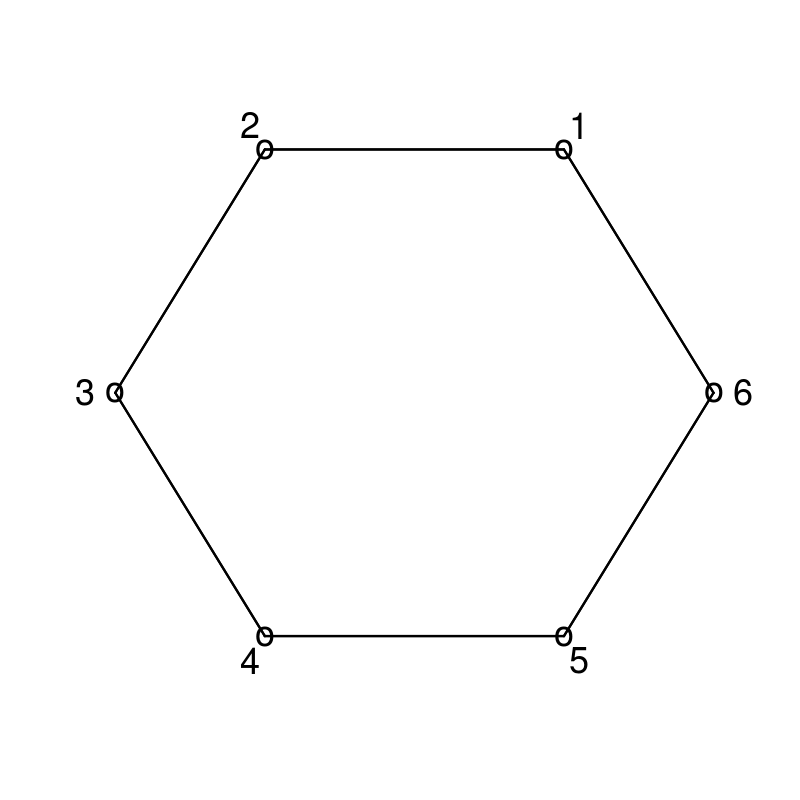
\includegraphics[scale = 0.3]{fig1_00.png}}
\end{tabular}
\end{frame}

\begin{frame}
\frametitle{Floyd-Warshall}
Iteration 1
\begin{tabular}{cc}
$
\begin{pmatrix}
0&1& & & &1\\
1&0&1& & &\blue[2]\\
 &1&0&1& & \\
 & &1&0&1& \\
 & & &1&0&1\\
1&\blue[2]& & &1&0\\
\end{pmatrix}
$
&
\raisebox{-.5\height}{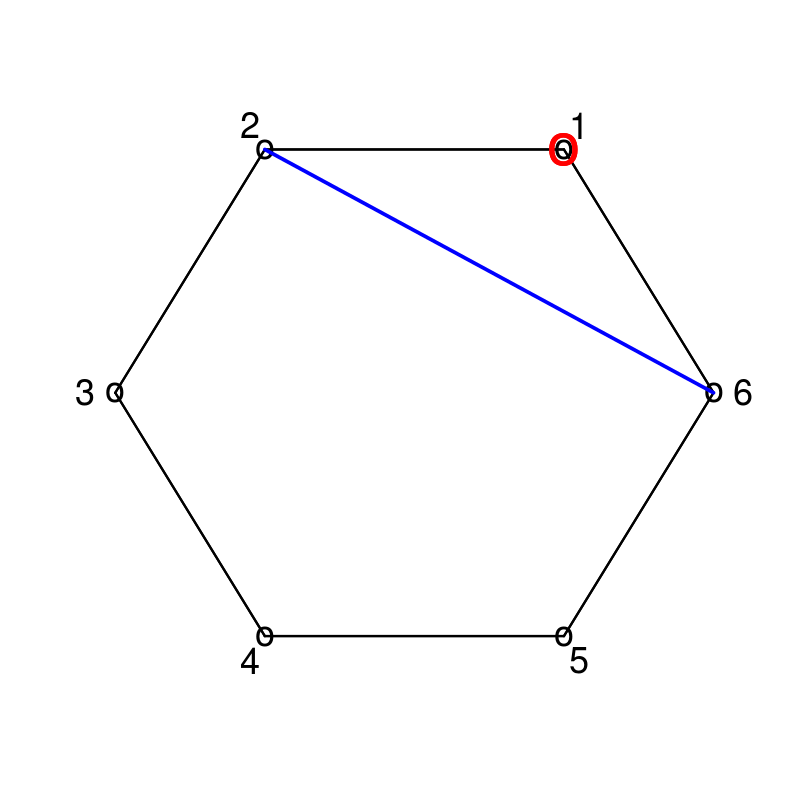
\includegraphics[scale = 0.3]{fig1_01.png}}
\end{tabular}
\end{frame}

\begin{frame}
\frametitle{Floyd-Warshall}
Iteration 2
\begin{tabular}{cc}
$
\begin{pmatrix}
0&1&\blue[2]& & &1\\
1&0&1& & &2\\
\blue[2]&1&0&1& &\blue[3]\\
 & &1&0&1& \\
 & & &1&0&1\\
1&2&\blue[3]& &1&0\\
\end{pmatrix}
$
&
\raisebox{-.5\height}{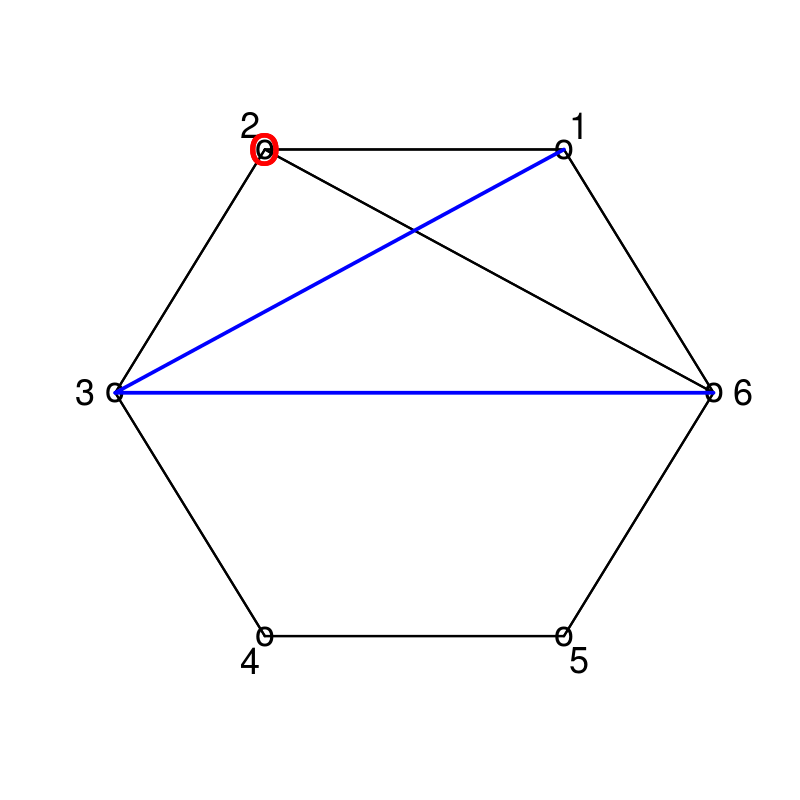
\includegraphics[scale = 0.3]{fig1_02.png}}
\end{tabular}
\end{frame}

\begin{frame}
\frametitle{Floyd-Warshall}
Iteration 3
\begin{tabular}{cc}
$
\begin{pmatrix}
0&1&2&\blue[3]& &1\\
1&0&1&\blue[2]& &2\\
2&1&0&1& &3\\
\blue[3]&\blue[2]&1&0&1&\blue[4]\\
 & & &1&0&1\\
1&2&3&\blue[4]&1&0\\
\end{pmatrix}
$
&
\raisebox{-.5\height}{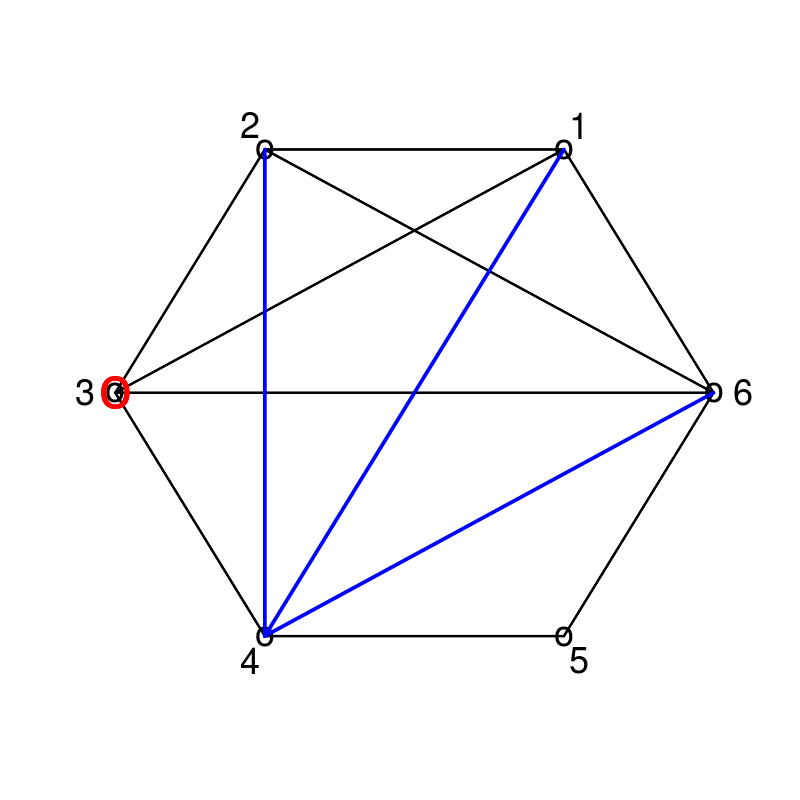
\includegraphics[scale = 0.3]{fig1_03.png}}
\end{tabular}
\end{frame}


\begin{frame}
\frametitle{Floyd-Warshall}
Iteration 4
\begin{tabular}{cc}
$
\begin{pmatrix}
0&1&2&3&\blue[4]&1\\
1&0&1&2&\blue[3]&2\\
2&1&0&1&\blue[2]&3\\
3&2&1&0&1&4\\
\blue[4]&\blue[3]&\blue[2]&1&0&1\\
1&2&3&4&1&0\\
\end{pmatrix}
$
&
\raisebox{-.5\height}{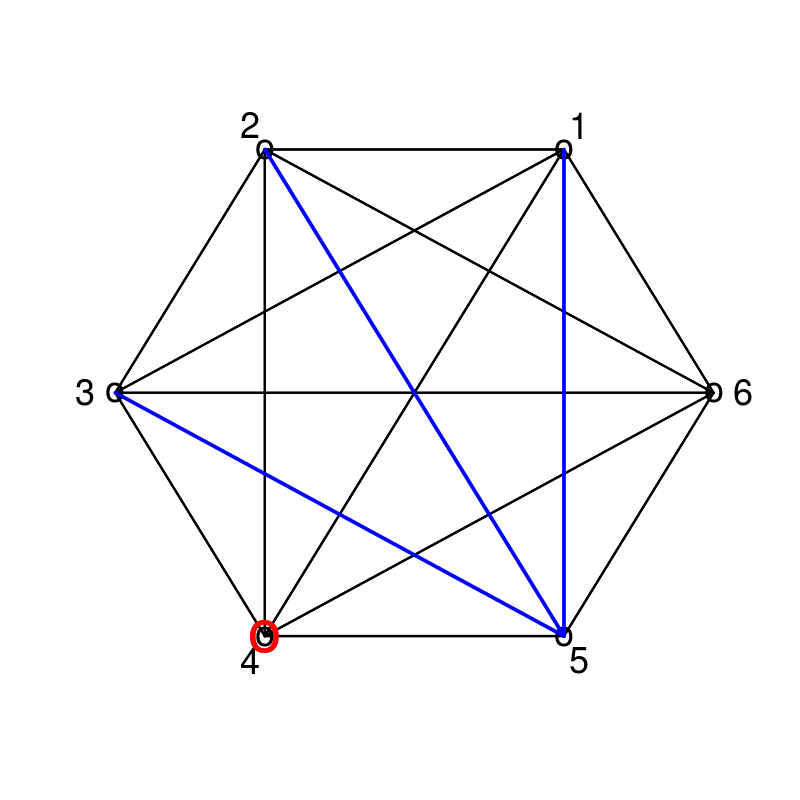
\includegraphics[scale = 0.3]{fig1_04.png}}
\end{tabular}
\end{frame}

\begin{frame}
\frametitle{Floyd-Warshall}
Iteration 5
\begin{tabular}{cc}
$
\begin{pmatrix}
0&1&2&3&4&1\\
1&0&1&2&3&2\\
2&1&0&1&2&3\\
3&2&1&0&1&\blue[2]\\
4&3&2&1&0&1\\
1&2&3&\blue[2]&1&0\\
\end{pmatrix}
$
&
\raisebox{-.5\height}{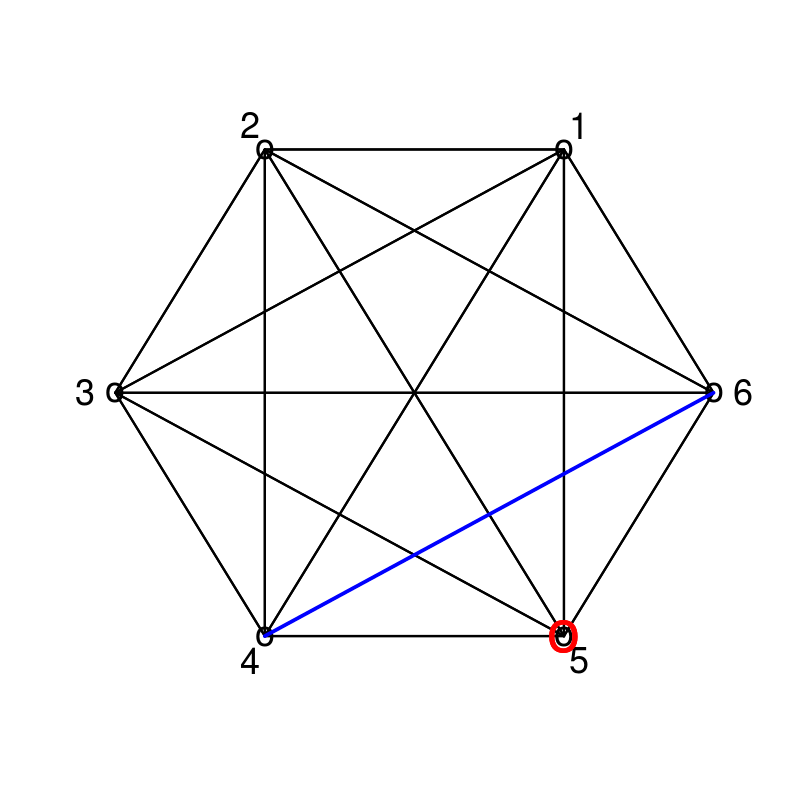
\includegraphics[scale = 0.3]{fig1_05.png}}
\end{tabular}
\end{frame}

\begin{frame}
\frametitle{Floyd-Warshall}
Iteration 6, \emph{(terminate)}
\begin{tabular}{cc}
$
\begin{pmatrix}
0&1&2&3&\blue[2]&1\\
1&0&1&2&3&2\\
2&1&0&1&2&3\\
3&2&1&0&1&2\\
\blue[2]&3&2&1&0&1\\
1&2&3&2&1&0\\
\end{pmatrix}
$
&
\raisebox{-.5\height}{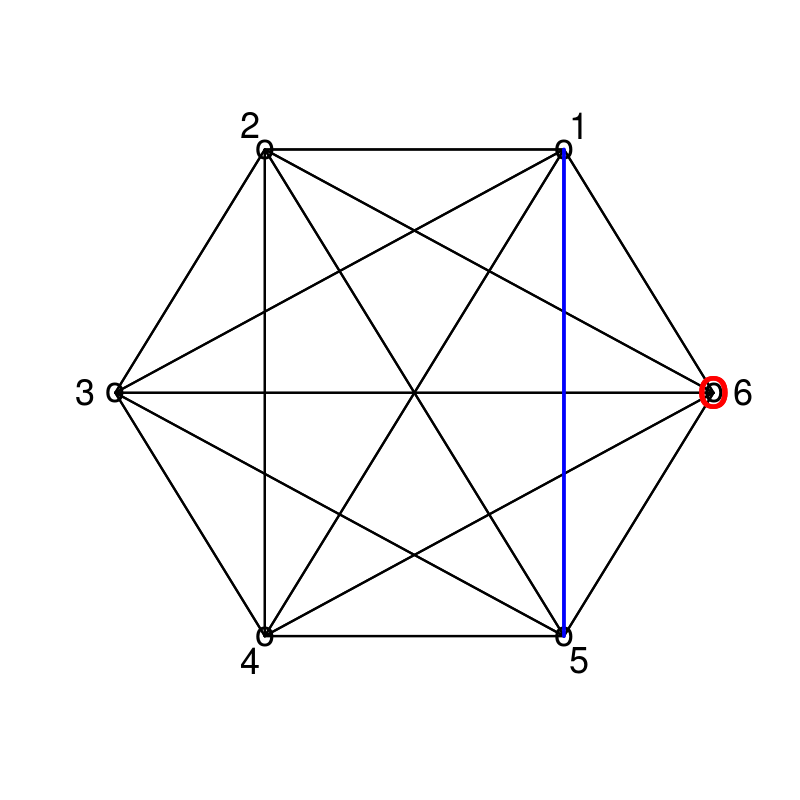
\includegraphics[scale = 0.3]{fig1_06.png}}
\end{tabular}
\end{frame}

\begin{frame}
\frametitle{Floyd-Warshall}
\begin{itemize}
\item Cost: $O(n^3)$ operations (single-core)
\item Takes $n$ \emph{sequential} iterations
\end{itemize}

\end{frame}

\begin{frame}
\frametitle{Problems with Floyd-Warshall}
\begin{itemize}
\item FW updates by considering 1 new vertex at a time
\item Result: $n$ iterations
\item High \# iterations = \emph{latency} in distributed setting
\item Solomonik et al. (2013) show how to ``block'' FW iterates
\item We modify their block-based approach for Spark
\end{itemize}
\end{frame}

\begin{frame}
\frametitle{Block APSP}
Number of vertices = $n$, Block Size = $b$
\begin{center}
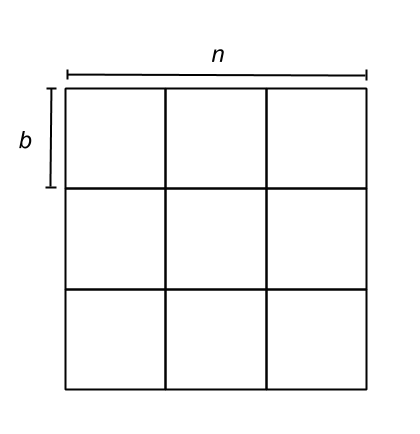
\includegraphics[scale = 0.4]{blockApsp-1.png}
\end{center}
\end{frame}

\begin{frame}
\frametitle{Block APSP}
Iteration 1A: Compute APSP within $V_1$ (block 1 on diagonal)
\begin{center}
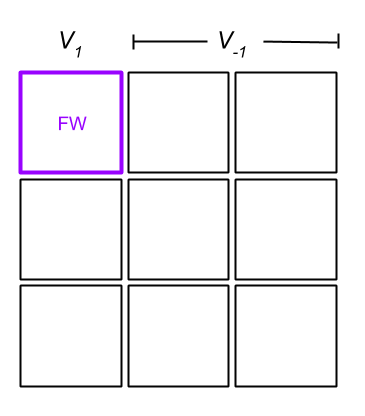
\includegraphics[scale = 0.4]{blockApsp-2.png}
\end{center}
\end{frame}

\begin{frame}
\frametitle{Block APSP}
Iteration 1B: Update weights of all paths to/from $V_1$
\begin{center}
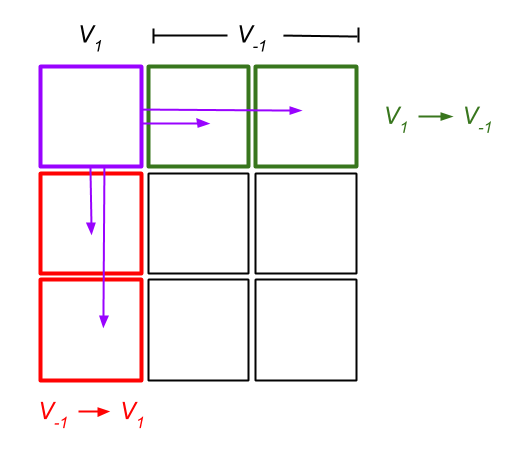
\includegraphics[scale = 0.4]{blockApsp-3.png}
\end{center}
\end{frame}

\begin{frame}
\frametitle{Block APSP}
Iteration 1C: Update weights of all paths starting and ending in $V_{-1}$ using
\[
S_{ij} \leftarrow min(S_{ij}, S_{ik} \otimes S_{kj}) \hspace{5mm} \text{where } k=1
\]
\begin{center}
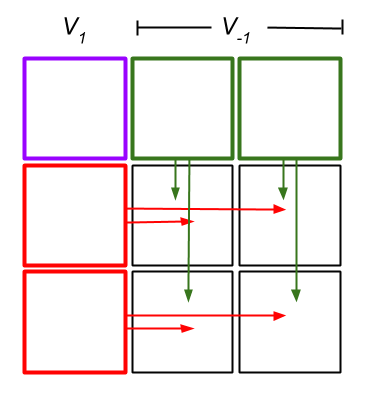
\includegraphics[scale = 0.4]{blockApsp-4.png}
\end{center}
\end{frame}


\begin{frame}
\frametitle{Block APSP}
Iteration 2: Do the same for block 2 on the diagonal
\begin{center}
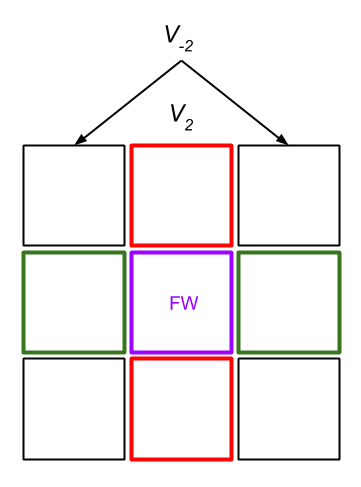
\includegraphics[scale = 0.4]{blockApsp-5.png}
\end{center}
\end{frame}

\begin{frame}
\frametitle{Block APSP: Single-core}
\begin{itemize}
\item Block size $b$, $n/b$ iterations 
\item A-step (all paths within block): $O(b^3)$
\item B-step (all paths to/from block): $O(nb^2)$
\item C-step (all paths through block): $O(n^2b)$
\item Iteration: $O(n^2 b + nb^2 + b^3)$
\item Total: $O(\frac{n}{b} (n^2 b + nb^2 + b^3)) = O(n^3 + n^2 b + nb^2)$
\item The case $b = 1$ is almost the same as Floyd-Warshall
\end{itemize}
\end{frame}

\begin{frame}
\frametitle{Distributing Block APSP}
\emph{Problem setup}
\begin{itemize}
\item Input format: Given by \emph{dense} adjacency matrix, stored as {\tt BlockMatrix} $S$ with block size $b$
\item Number of vertices $n$ is large
\item Output format: same
\item Each block fits in memory
\end{itemize}
\end{frame}

\begin{frame}
\frametitle{Distributing Block APSP}
For $i = 1,\hdots, n/b$
\begin{itemize}
\item A-step: \emph{(update all paths within block)}
\begin{itemize}
\item One-to-one communication
\item Computation $O(b^3)$
\item Bandwidth $O(b^2)$
\item Runtime $O(b^3)$
\end{itemize} 
\end{itemize}
\begin{center}
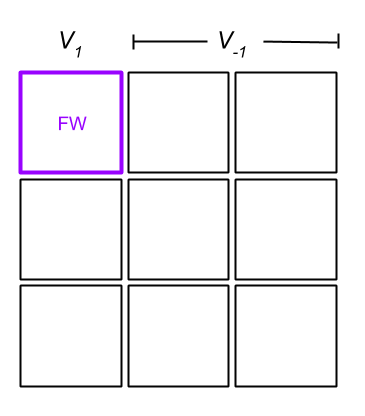
\includegraphics[scale = 0.3]{blockApsp-2.png}
\end{center}
\end{frame}

\begin{frame}
\frametitle{Distributing Block APSP}
\begin{itemize}
\item B-step: \emph{(update all paths to/from block)}
\begin{itemize}
\item One-to-all communication
\item Computation per worker: $O(nb^2/\sqrt{p})$
\item Bandwidth $O(b^2 \sqrt{p})$
\item Runtime $O(\log(p)b^2 + b^2n/\sqrt{p})$
\end{itemize}
\end{itemize}
\begin{center}
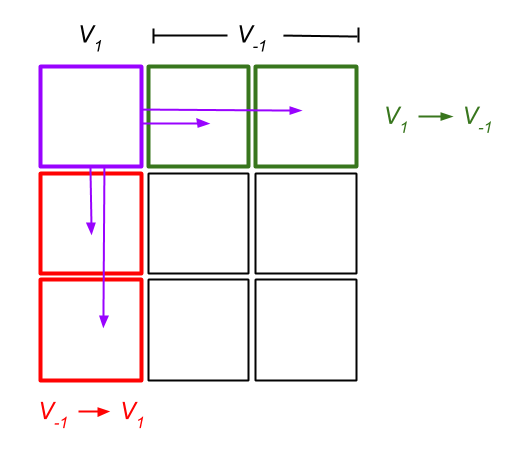
\includegraphics[scale = 0.3]{blockApsp-3.png}
\end{center}
\end{frame}

\begin{frame}
\frametitle{Distributing Block APSP}
\begin{itemize}
\item C-step: \emph{(update all paths through block)}
\begin{itemize}
\item All-to-all communication
\item Computation per worker: $O(n^2b/p)$
\item Bandwidth: $O(nb\sqrt{p})$
\item Runtime: $O(n^2b/p  + nb)$
\end{itemize}
\end{itemize}
\begin{center}
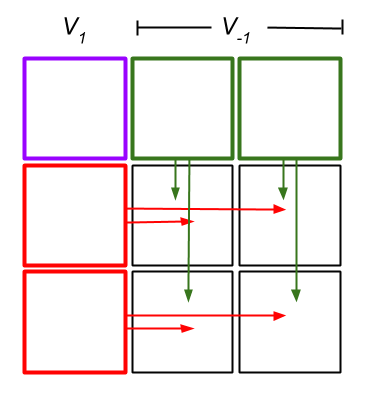
\includegraphics[scale = 0.3]{blockApsp-4.png}
\end{center}

\end{frame}

\begin{frame}
\frametitle{Distributing Block APSP}
Overall cost:
\begin{itemize}
\item Total computational cost is $O(n^3 + n^2b)$ divided evenly among workers plus $O(nb^2)$ on driver
\item Total communication cost: $O(n^2\sqrt{p})$
\item Total runtime: $O(\frac{n^3}{p} + \frac{n^2 b}{\sqrt{p}} +  n^2 + nb^2 + nb\log(p))$
\end{itemize}
Ignoring latency, optimal $b= 1$\\

With latency, runtime is
\[
\frac{n}{b}L + K\left(nb^2+ \left(n\log(p) + \frac{n^2}{\sqrt{p}}\right)b +\frac{n^3}{p}  +  n^2 \right)
\]
so $b \neq 1$ may be optimal
\end{frame}

\begin{frame}
\frametitle{More Implementation details on Spark}
\begin{itemize}
\item Grid Partitioner
\item Checkpointing

\end{itemize}
\end{frame}

\begin{frame}
\frametitle{Results}
n = 500, p = 4; Local[4] 8GB
\begin{center}
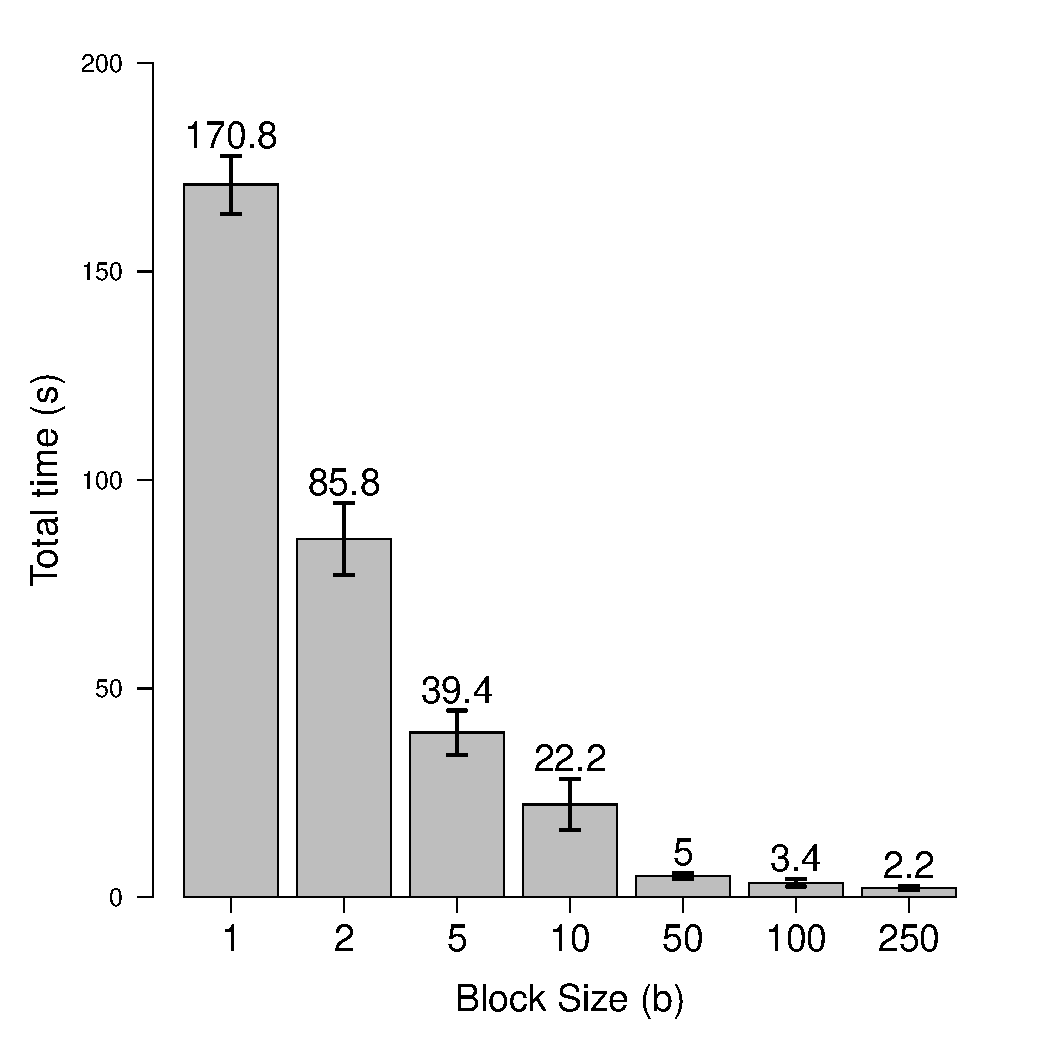
\includegraphics[scale = 0.4]{time.pdf}
\end{center}

\end{frame}

\begin{frame}
\begin{center}
Thank you!
\end{center}
\end{frame}


\end{document}
